\documentclass[11pt,a4paper]{article}
\usepackage{lmodern}
\usepackage{amssymb,amsmath}
\usepackage{ifxetex,ifluatex}
\usepackage{fixltx2e} % provides \textsubscript
\ifnum 0\ifxetex 1\fi\ifluatex 1\fi=0 % if pdftex
  \usepackage[T1]{fontenc}
  \usepackage[utf8]{inputenc}
\else % if luatex or xelatex
  \ifxetex
    \usepackage{mathspec}
  \else
    \usepackage{fontspec}
  \fi
  \defaultfontfeatures{Ligatures=TeX,Scale=MatchLowercase}
\fi
% use upquote if available, for straight quotes in verbatim environments
\IfFileExists{upquote.sty}{\usepackage{upquote}}{}
% use microtype if available
\IfFileExists{microtype.sty}{%
\usepackage{microtype}
\UseMicrotypeSet[protrusion]{basicmath} % disable protrusion for tt fonts
}{}
\usepackage[margin=2cm]{geometry}
\usepackage{hyperref}
\hypersetup{unicode=true,
            pdftitle={Notes on S3M sampling},
            pdfborder={0 0 0},
            breaklinks=true}
\urlstyle{same}  % don't use monospace font for urls
\usepackage{color}
\usepackage{fancyvrb}
\newcommand{\VerbBar}{|}
\newcommand{\VERB}{\Verb[commandchars=\\\{\}]}
\DefineVerbatimEnvironment{Highlighting}{Verbatim}{commandchars=\\\{\}}
% Add ',fontsize=\small' for more characters per line
\newenvironment{Shaded}{}{}
\newcommand{\KeywordTok}[1]{\textcolor[rgb]{0.00,0.44,0.13}{\textbf{#1}}}
\newcommand{\DataTypeTok}[1]{\textcolor[rgb]{0.56,0.13,0.00}{#1}}
\newcommand{\DecValTok}[1]{\textcolor[rgb]{0.25,0.63,0.44}{#1}}
\newcommand{\BaseNTok}[1]{\textcolor[rgb]{0.25,0.63,0.44}{#1}}
\newcommand{\FloatTok}[1]{\textcolor[rgb]{0.25,0.63,0.44}{#1}}
\newcommand{\ConstantTok}[1]{\textcolor[rgb]{0.53,0.00,0.00}{#1}}
\newcommand{\CharTok}[1]{\textcolor[rgb]{0.25,0.44,0.63}{#1}}
\newcommand{\SpecialCharTok}[1]{\textcolor[rgb]{0.25,0.44,0.63}{#1}}
\newcommand{\StringTok}[1]{\textcolor[rgb]{0.25,0.44,0.63}{#1}}
\newcommand{\VerbatimStringTok}[1]{\textcolor[rgb]{0.25,0.44,0.63}{#1}}
\newcommand{\SpecialStringTok}[1]{\textcolor[rgb]{0.73,0.40,0.53}{#1}}
\newcommand{\ImportTok}[1]{#1}
\newcommand{\CommentTok}[1]{\textcolor[rgb]{0.38,0.63,0.69}{\textit{#1}}}
\newcommand{\DocumentationTok}[1]{\textcolor[rgb]{0.73,0.13,0.13}{\textit{#1}}}
\newcommand{\AnnotationTok}[1]{\textcolor[rgb]{0.38,0.63,0.69}{\textbf{\textit{#1}}}}
\newcommand{\CommentVarTok}[1]{\textcolor[rgb]{0.38,0.63,0.69}{\textbf{\textit{#1}}}}
\newcommand{\OtherTok}[1]{\textcolor[rgb]{0.00,0.44,0.13}{#1}}
\newcommand{\FunctionTok}[1]{\textcolor[rgb]{0.02,0.16,0.49}{#1}}
\newcommand{\VariableTok}[1]{\textcolor[rgb]{0.10,0.09,0.49}{#1}}
\newcommand{\ControlFlowTok}[1]{\textcolor[rgb]{0.00,0.44,0.13}{\textbf{#1}}}
\newcommand{\OperatorTok}[1]{\textcolor[rgb]{0.40,0.40,0.40}{#1}}
\newcommand{\BuiltInTok}[1]{#1}
\newcommand{\ExtensionTok}[1]{#1}
\newcommand{\PreprocessorTok}[1]{\textcolor[rgb]{0.74,0.48,0.00}{#1}}
\newcommand{\AttributeTok}[1]{\textcolor[rgb]{0.49,0.56,0.16}{#1}}
\newcommand{\RegionMarkerTok}[1]{#1}
\newcommand{\InformationTok}[1]{\textcolor[rgb]{0.38,0.63,0.69}{\textbf{\textit{#1}}}}
\newcommand{\WarningTok}[1]{\textcolor[rgb]{0.38,0.63,0.69}{\textbf{\textit{#1}}}}
\newcommand{\AlertTok}[1]{\textcolor[rgb]{1.00,0.00,0.00}{\textbf{#1}}}
\newcommand{\ErrorTok}[1]{\textcolor[rgb]{1.00,0.00,0.00}{\textbf{#1}}}
\newcommand{\NormalTok}[1]{#1}
\usepackage{longtable,booktabs}
\usepackage{graphicx,grffile}
\makeatletter
\def\maxwidth{\ifdim\Gin@nat@width>\linewidth\linewidth\else\Gin@nat@width\fi}
\def\maxheight{\ifdim\Gin@nat@height>\textheight\textheight\else\Gin@nat@height\fi}
\makeatother
% Scale images if necessary, so that they will not overflow the page
% margins by default, and it is still possible to overwrite the defaults
% using explicit options in \includegraphics[width, height, ...]{}
\setkeys{Gin}{width=\maxwidth,height=\maxheight,keepaspectratio}
\IfFileExists{parskip.sty}{%
\usepackage{parskip}
}{% else
\setlength{\parindent}{0pt}
\setlength{\parskip}{6pt plus 2pt minus 1pt}
}
\setlength{\emergencystretch}{3em}  % prevent overfull lines
\providecommand{\tightlist}{%
  \setlength{\itemsep}{0pt}\setlength{\parskip}{0pt}}
\setcounter{secnumdepth}{0}
% Redefines (sub)paragraphs to behave more like sections
\ifx\paragraph\undefined\else
\let\oldparagraph\paragraph
\renewcommand{\paragraph}[1]{\oldparagraph{#1}\mbox{}}
\fi
\ifx\subparagraph\undefined\else
\let\oldsubparagraph\subparagraph
\renewcommand{\subparagraph}[1]{\oldsubparagraph{#1}\mbox{}}
\fi

%%% Use protect on footnotes to avoid problems with footnotes in titles
\let\rmarkdownfootnote\footnote%
\def\footnote{\protect\rmarkdownfootnote}

%%% Change title format to be more compact
\usepackage{titling}

% Create subtitle command for use in maketitle
\newcommand{\subtitle}[1]{
  \posttitle{
    \begin{center}\large#1\end{center}
    }
}

\setlength{\droptitle}{-2em}
  \title{Notes on S3M sampling}
  \pretitle{\vspace{\droptitle}\centering\huge}
  \posttitle{\par}
  \author{}
  \preauthor{}\postauthor{}
  \predate{\centering\large\emph}
  \postdate{\par}
  \date{10 June 2018}


\begin{document}
\maketitle

\hypertarget{warning-message-when-reading-boundary-shapefiles}{%
\subsection{1. Warning message when reading boundary
shapefiles}\label{warning-message-when-reading-boundary-shapefiles}}

In \texttt{Read\ map\ data} node, you get the following warning
messages:

~

\begin{Shaded}
\begin{Highlighting}[]
\NormalTok{st <-}\StringTok{ }\KeywordTok{readShapeSpatial}\NormalTok{(}\StringTok{"Boundary_Shapefiles/02_StateBoundaries_Poly_2013.shp"}\NormalTok{, }
                       \DataTypeTok{proj4string =} \KeywordTok{CRS}\NormalTok{(}\StringTok{"+proj=longlat +dataum=WGS84"}\NormalTok{))}
\end{Highlighting}
\end{Shaded}

\begin{verbatim}
## Warning: use rgdal::readOGR or sf::st_read

## Warning: use rgdal::readOGR or sf::st_read
\end{verbatim}

~

\begin{Shaded}
\begin{Highlighting}[]
\NormalTok{loc1 <-}\StringTok{ }\KeywordTok{readShapeSpatial}\NormalTok{(}\StringTok{"Boundary_Shapefiles/03_Locality_Boundaries_Poly_2013.shp"}\NormalTok{, }
                         \DataTypeTok{proj4string =} \KeywordTok{CRS}\NormalTok{(}\StringTok{"+proj=longlat +dataum=WGS84"}\NormalTok{))}
\end{Highlighting}
\end{Shaded}

\begin{verbatim}
## Warning: use rgdal::readOGR or sf::st_read

## Warning: use rgdal::readOGR or sf::st_read
\end{verbatim}

~

The \texttt{readShapeSpatial()} function in package \texttt{maptools} is
scheduled for deprecation and has now been superseded by the
\texttt{readOGR()} function in package \texttt{rgdal} (written by the
same author). Since the first Sudan S3M, we have shifted our mapping
libraries away from \texttt{maptools} and into \texttt{rgdal}. The main
differentiating features of \texttt{readOGR()} is that it actually
detects/reads the projection ascribed to a Shapefile without having to
be specified (as what is needed for \texttt{readShapeSpatial()}) and
that it can read about 8 other geographic formats (i.e., kml,
gpx\ldots{}). I would recommend that we do the same for this current
workflow and for future S3M workflows.

To read the same files using \texttt{readOGR()}, we use the following
syntax:

~

\begin{Shaded}
\begin{Highlighting}[]
\NormalTok{st <-}\StringTok{ }\KeywordTok{readOGR}\NormalTok{(}\DataTypeTok{dsn =} \StringTok{"Boundary_Shapefiles"}\NormalTok{,            }\CommentTok{# directory containing SHP}
              \DataTypeTok{layer =} \StringTok{"02_StateBoundaries_Poly_2013"}\NormalTok{) }\CommentTok{# name of the SHP layer}
\end{Highlighting}
\end{Shaded}

\begin{verbatim}
## OGR data source with driver: ESRI Shapefile 
## Source: "/Users/ernest/Dropbox/R/S3M/new/s3mTRI/Boundary_Shapefiles", layer: "02_StateBoundaries_Poly_2013"
## with 18 features
## It has 4 fields
\end{verbatim}

~

You can remove the message output describing the geodata that has just
been read by adding the \texttt{verbose} argument and setting it to
\texttt{FALSE}:

\begin{Shaded}
\begin{Highlighting}[]
\NormalTok{st <-}\StringTok{ }\KeywordTok{readOGR}\NormalTok{(}\DataTypeTok{dsn =} \StringTok{"Boundary_Shapefiles"}\NormalTok{,}
              \DataTypeTok{layer =} \StringTok{"02_StateBoundaries_Poly_2013"}\NormalTok{,}
              \DataTypeTok{verbose =} \OtherTok{FALSE}\NormalTok{)}
\end{Highlighting}
\end{Shaded}

~

You will notice that if you check for the project of the
\texttt{SpatialPolygonsDataFrame} object created by \texttt{readOGR()},
it will show:

~

\begin{Shaded}
\begin{Highlighting}[]
\KeywordTok{proj4string}\NormalTok{(st)}
\end{Highlighting}
\end{Shaded}

\begin{verbatim}
## [1] "+proj=longlat +datum=WGS84 +no_defs +ellps=WGS84 +towgs84=0,0,0"
\end{verbatim}

~

The \texttt{SpatialPolygonsDataFrame} object \texttt{st} has been
assigned the appropriate projection.

\newpage

\hypertarget{consider-other-relevant-geospatial-libraries}{%
\subsection{2. Consider other relevant geospatial
libraries}\label{consider-other-relevant-geospatial-libraries}}

I would suggesting a few relevant geospatial libraries that I think,
based on experience, have really good functions that help with
manipulating geospatial data.

\hypertarget{a.-rgdal}{%
\subsubsection{\texorpdfstring{a.
\texttt{rgdal}}{a. rgdal}}\label{a.-rgdal}}

As commented above, I would suggest adding this and using its read and
write functions for geospatial data;

\hypertarget{b.-raster}{%
\subsubsection{\texorpdfstring{b.
\texttt{raster}}{b. raster}}\label{b.-raster}}

I looked at the node for the function libraries and \texttt{raster} was
included there before. We included that before not becuase we are using
raster data but mainly for two general features:

\begin{itemize}
\item
  \texttt{raster} package when installed alongside \texttt{rgdal} and
  \texttt{rgeos} allows for more efficient onloading and offloading of
  geospatial data. What I mean by this is that it faciliates ``lazy''
  handling especially of big (in terms of memory size and of actual
  fields and features) geospatial data.
\item
  \texttt{raster} package includes utility geospatial functions found in
  standard GIS packages that we might consider using for some
  functionalities that I think we might want consider for S3M based on
  my further comments below. Some examples of these functions are
  \texttt{intersect()}, \texttt{union()}, \texttt{difference()}.
\item
  \texttt{geosphere} - I notice that we use \texttt{Imap} package mainly
  to use the \texttt{gdist()} function. I was wondering whether it would
  be better to use the \texttt{geosphere()} package which is a purely
  distance calculatur package and the functions are highly vectorised so
  they are very efficient (see comment below on \texttt{gdist()}
  warning). The other thinking to consider here will be whether we
  actually need to use a geodesic distance calculator for finding
  nearest village or any other distance calculation requirements down
  the line. It might be that we consider Euclidean approaches to
  distance calculation? They tend to be faster to implement, highly
  vectorised. I am thinking functions that include finidng nearest
  neighbour algorithm works well. The \texttt{gstat} package that we use
  for spatial interpolation uses \texttt{FNN} package for its nearest
  neighbour search for its \texttt{idw()} function. We also use the
  \texttt{FNN} package for our cross-validation functions for spatial
  interpolation.
\end{itemize}

\newpage

\hypertarget{warning-message-when-applying-nearestpoint-function}{%
\subsection{\texorpdfstring{3. Warning message when applying
\texttt{nearestPoint()}
function}{3. Warning message when applying nearestPoint() function}}\label{warning-message-when-applying-nearestpoint-function}}

In the node for \texttt{State\ Grid\ TRI} and
\texttt{Locality\ Grid\ TRI}, there are multiple warnings that show up
when the \texttt{nearestPoint()} function as applied:

~

\begin{Shaded}
\begin{Highlighting}[]
\NormalTok{selPS <-}\StringTok{ }\KeywordTok{nearestPoint}\NormalTok{(SPs, vil)}
\end{Highlighting}
\end{Shaded}

\begin{verbatim}
## Warning in while (abs(lamda - lamda.old) > 1e-11) {: the condition has
## length > 1 and only the first element will be used

## Warning in while (abs(lamda - lamda.old) > 1e-11) {: the condition has
## length > 1 and only the first element will be used

## Warning in while (abs(lamda - lamda.old) > 1e-11) {: the condition has
## length > 1 and only the first element will be used

## Warning in while (abs(lamda - lamda.old) > 1e-11) {: the condition has
## length > 1 and only the first element will be used

## Warning in while (abs(lamda - lamda.old) > 1e-11) {: the condition has
## length > 1 and only the first element will be used

## Warning in while (abs(lamda - lamda.old) > 1e-11) {: the condition has
## length > 1 and only the first element will be used

## Warning in while (abs(lamda - lamda.old) > 1e-11) {: the condition has
## length > 1 and only the first element will be used

## Warning in while (abs(lamda - lamda.old) > 1e-11) {: the condition has
## length > 1 and only the first element will be used

## Warning in while (abs(lamda - lamda.old) > 1e-11) {: the condition has
## length > 1 and only the first element will be used

## Warning in while (abs(lamda - lamda.old) > 1e-11) {: the condition has
## length > 1 and only the first element will be used

## Warning in while (abs(lamda - lamda.old) > 1e-11) {: the condition has
## length > 1 and only the first element will be used

## Warning in while (abs(lamda - lamda.old) > 1e-11) {: the condition has
## length > 1 and only the first element will be used

## Warning in while (abs(lamda - lamda.old) > 1e-11) {: the condition has
## length > 1 and only the first element will be used

## Warning in while (abs(lamda - lamda.old) > 1e-11) {: the condition has
## length > 1 and only the first element will be used

## Warning in while (abs(lamda - lamda.old) > 1e-11) {: the condition has
## length > 1 and only the first element will be used

## Warning in while (abs(lamda - lamda.old) > 1e-11) {: the condition has
## length > 1 and only the first element will be used

## Warning in while (abs(lamda - lamda.old) > 1e-11) {: the condition has
## length > 1 and only the first element will be used

## Warning in while (abs(lamda - lamda.old) > 1e-11) {: the condition has
## length > 1 and only the first element will be used

## Warning in while (abs(lamda - lamda.old) > 1e-11) {: the condition has
## length > 1 and only the first element will be used

## Warning in while (abs(lamda - lamda.old) > 1e-11) {: the condition has
## length > 1 and only the first element will be used
\end{verbatim}

~

Despite the warning, the resulting object \texttt{selPS} contains the
data frame that is expected.

~

\begin{Shaded}
\begin{Highlighting}[]
\NormalTok{selPS}
\end{Highlighting}
\end{Shaded}

\begin{verbatim}
##    id        x        y         village             locality
## 1 920 33.28083 12.61028  Galaa' AlBeid' AlDali and AlMazmoum
## 2  54 34.14706 12.64006  Wad Girif Awal            Abu Hijar
## 3 244 34.79008 12.82597  Um Bagara Garb            Al Dindir
## 4 939 33.67212 13.45171 Wad Hashim Mroa               Sennar
##                    d
## 1   8.39494441502051
## 2 0.0534743139366605
## 3   38.0782315663253
## 4  0.678767494050234
\end{verbatim}

~

This warning is most likely coming from the application of the
\texttt{gdist()} function within the \texttt{nearestPoint()} function.

\texttt{gdist()} requires single value inputs for \texttt{lon.1},
\texttt{lat.1}, \texttt{lon.2}, \texttt{lat.2} arguments. In the
\texttt{nearestPoint()} function however, the \texttt{x} and \texttt{y}
arguments are expected to be vectors and \texttt{gdist()} function is
supplied a vector for \texttt{lon.2} and \texttt{lat.2} arguments.
Despite this, the \texttt{gdist()} function is able to deal with this
mainly because its application of the distance calculation is vectorised
and R by default just addresses the problem by using the first values in
the \texttt{lon.2} and \texttt{lat.2} vectors. So, as suggested in the
workflow, it seems this warning can be safely ignored.

Ideally, the best solution to this would be for the \texttt{gdist()}
function to be udpated and that the longitude and latitude coordinate
inputs be vectorised as default rather than single values.

I wonder, however, whether we would want to update
\texttt{nearestPoint()} so that it can deal with the limitations of the
\texttt{gist()} function or that we change the geodesic distance
calculator function that we are using. This is related to my comment
earlier about the use of the functions in the \texttt{geosphere()}
package instead or just using a Euclidean distance calculation from a
basis nearest neighbour algorithm.

Below is an example of how we can update \texttt{nearestPoint()} by
vectorising the application of the \texttt{gdist()}:

~

\begin{Shaded}
\begin{Highlighting}[]
\NormalTok{nearestPoint <-}\StringTok{ }\ControlFlowTok{function}\NormalTok{(x, y) \{}
\NormalTok{  near.point <-}\StringTok{ }\OtherTok{NULL}
    \ControlFlowTok{for}\NormalTok{(i }\ControlFlowTok{in} \DecValTok{1}\OperatorTok{:}\KeywordTok{length}\NormalTok{(x)) \{}
\NormalTok{      near.point1 <-}\StringTok{ }\KeywordTok{mapply}\NormalTok{(}\DataTypeTok{FUN =}\NormalTok{ gdist, }\DataTypeTok{lon.2 =}\NormalTok{ y[ , }\DecValTok{2}\NormalTok{], }\DataTypeTok{lat.2 =}\NormalTok{ y[ , }\DecValTok{3}\NormalTok{],}
                          \DataTypeTok{MoreArgs =} \KeywordTok{list}\NormalTok{(x}\OperatorTok{$}\NormalTok{x[i], x}\OperatorTok{$}\NormalTok{y[i], }\DataTypeTok{units =} \StringTok{"km"}\NormalTok{))}
        
\NormalTok{        near.point2 <-}\StringTok{ }\KeywordTok{c}\NormalTok{(y}\OperatorTok{$}\NormalTok{id[}\KeywordTok{which}\NormalTok{(near.point1 }\OperatorTok{==}\StringTok{ }\KeywordTok{min}\NormalTok{(near.point1))], }
\NormalTok{                                     y}\OperatorTok{$}\NormalTok{x[}\KeywordTok{which}\NormalTok{(near.point1 }\OperatorTok{==}\StringTok{ }\KeywordTok{min}\NormalTok{(near.point1))], }
\NormalTok{                                   y}\OperatorTok{$}\NormalTok{y[}\KeywordTok{which}\NormalTok{(near.point1 }\OperatorTok{==}\StringTok{ }\KeywordTok{min}\NormalTok{(near.point1))], }
\NormalTok{                                   y}\OperatorTok{$}\NormalTok{village[}\KeywordTok{which}\NormalTok{(near.point1 }\OperatorTok{==}\StringTok{ }\KeywordTok{min}\NormalTok{(near.point1))], }
\NormalTok{                                   y}\OperatorTok{$}\NormalTok{locality[}\KeywordTok{which}\NormalTok{(near.point1 }\OperatorTok{==}\StringTok{ }\KeywordTok{min}\NormalTok{(near.point1))], }
                                   \KeywordTok{min}\NormalTok{(near.point1))}
        
\NormalTok{      near.point <-}\StringTok{ }\KeywordTok{rbind}\NormalTok{(near.point, near.point2)}
\NormalTok{    \}}
\NormalTok{  near.point <-}\StringTok{ }\KeywordTok{as.data.frame}\NormalTok{(near.point)}
    \KeywordTok{names}\NormalTok{(near.point) <-}\StringTok{ }\KeywordTok{c}\NormalTok{(}\StringTok{"id"}\NormalTok{, }\StringTok{"x"}\NormalTok{, }\StringTok{"y"}\NormalTok{, }\StringTok{"village"}\NormalTok{, }\StringTok{"locality"}\NormalTok{, }\StringTok{"d"}\NormalTok{) }
    \KeywordTok{rownames}\NormalTok{(near.point) <-}\StringTok{ }\OtherTok{NULL}  
\NormalTok{    near.point[,}\DecValTok{1}\NormalTok{] <-}\StringTok{ }\KeywordTok{as.numeric}\NormalTok{(near.point[,}\DecValTok{1}\NormalTok{])}
\NormalTok{    near.point[,}\DecValTok{2}\NormalTok{] <-}\StringTok{ }\KeywordTok{as.numeric}\NormalTok{(near.point[,}\DecValTok{2}\NormalTok{])}
\NormalTok{    near.point[,}\DecValTok{3}\NormalTok{] <-}\StringTok{ }\KeywordTok{as.numeric}\NormalTok{(near.point[,}\DecValTok{3}\NormalTok{]) }
\NormalTok{    near.point <-}\StringTok{ }\NormalTok{near.point[}\OperatorTok{!}\KeywordTok{duplicated}\NormalTok{(near.point[,}\OperatorTok{-}\DecValTok{6}\NormalTok{]),]}
    \KeywordTok{return}\NormalTok{(near.point)}
\NormalTok{\}}
\end{Highlighting}
\end{Shaded}

~

Here all I have done is to edit the line where we apply the
\texttt{gdist()} function by simply using it inside \texttt{mapply()} so
that it can be applied to every row of values in the vector of community
location coordinates.

When we apply the udpate \texttt{nearestPoint()} function, we get no
warnings and we get the same results.

~

\begin{Shaded}
\begin{Highlighting}[]
\NormalTok{selPS <-}\StringTok{ }\KeywordTok{nearestPoint}\NormalTok{(SPs, vil)}
\NormalTok{selPS}
\end{Highlighting}
\end{Shaded}

\begin{verbatim}
##    id        x        y         village             locality
## 1 920 33.28083 12.61028  Galaa' AlBeid' AlDali and AlMazmoum
## 2  54 34.14706 12.64006  Wad Girif Awal            Abu Hijar
## 3 244 34.79008 12.82597  Um Bagara Garb            Al Dindir
## 4 939 33.67212 13.45171 Wad Hashim Mroa               Sennar
##                   d
## 1  8.39494441502051
## 2 0.053474313755245
## 3  38.0782315663253
## 4 0.678767472454879
\end{verbatim}

~

Trying out the Euclidean distance calculations found in package
\texttt{FNN}, we can use the following function:

~

\begin{Shaded}
\begin{Highlighting}[]
\NormalTok{get_nn <-}\StringTok{ }\ControlFlowTok{function}\NormalTok{(data, x1, y1, query, x2, y2, n) \{}
\NormalTok{  near.index <-}\StringTok{ }\KeywordTok{get.knnx}\NormalTok{(}\DataTypeTok{data =}\NormalTok{ data[ , }\KeywordTok{c}\NormalTok{(x1, y1)], }
                         \DataTypeTok{query =}\NormalTok{ query[ , }\KeywordTok{c}\NormalTok{(x2, y2)], }
                         \DataTypeTok{k =}\NormalTok{ n)}
\NormalTok{  near.point <-}\StringTok{ }\NormalTok{data[near.index}\OperatorTok{$}\NormalTok{nn.index, ]}
\NormalTok{  near.point <-}\StringTok{ }\KeywordTok{data.frame}\NormalTok{(near.point, }\DataTypeTok{d =} \KeywordTok{c}\NormalTok{(near.index}\OperatorTok{$}\NormalTok{nn.dist))  }
\NormalTok{  near.point <-}\StringTok{ }\NormalTok{near.point[}\OperatorTok{!}\KeywordTok{duplicated}\NormalTok{(near.point[ , }\KeywordTok{c}\NormalTok{(x1, y1)]), ]}
  \KeywordTok{row.names}\NormalTok{(near.point) <-}\StringTok{ }\DecValTok{1}\OperatorTok{:}\KeywordTok{nrow}\NormalTok{(near.point)}
  \KeywordTok{return}\NormalTok{(near.point)}
\NormalTok{\}}
\end{Highlighting}
\end{Shaded}

~

where:

~

\begin{longtable}[]{@{}rl@{}}
\toprule
\begin{minipage}[t]{0.10\columnwidth}\raggedleft
data\strut
\end{minipage} & \begin{minipage}[t]{0.82\columnwidth}\raggedright
an input data frame or matrix containing longitude and latitude
coordinate of village locations\strut
\end{minipage}\tabularnewline
\begin{minipage}[t]{0.10\columnwidth}\raggedleft
x1\strut
\end{minipage} & \begin{minipage}[t]{0.82\columnwidth}\raggedright
a character value specifying the variable name in \texttt{data} holding
the longitude and latitude coordinate of village locations\strut
\end{minipage}\tabularnewline
\begin{minipage}[t]{0.10\columnwidth}\raggedleft
y1\strut
\end{minipage} & \begin{minipage}[t]{0.82\columnwidth}\raggedright
a character value specifying the variable name in \texttt{data} holding
the latitude coordinate values\strut
\end{minipage}\tabularnewline
\begin{minipage}[t]{0.10\columnwidth}\raggedleft
query\strut
\end{minipage} & \begin{minipage}[t]{0.82\columnwidth}\raggedright
an object of class \texttt{SpatialPoints} containing sampling point
locations. This is usually the output from applying \texttt{spsample()}
function from package \texttt{gstat} to create an even spatial across
the entire sampling area\strut
\end{minipage}\tabularnewline
\begin{minipage}[t]{0.10\columnwidth}\raggedleft
x2\strut
\end{minipage} & \begin{minipage}[t]{0.82\columnwidth}\raggedright
a character value specifying the variable name in holding the longitude
coordinate values\strut
\end{minipage}\tabularnewline
\begin{minipage}[t]{0.10\columnwidth}\raggedleft
y2\strut
\end{minipage} & \begin{minipage}[t]{0.82\columnwidth}\raggedright
a character value specifying the variable name in query holding the
latitude coordinate values\strut
\end{minipage}\tabularnewline
\begin{minipage}[t]{0.10\columnwidth}\raggedleft
n\strut
\end{minipage} & \begin{minipage}[t]{0.82\columnwidth}\raggedright
number of nearest neighbours to search\strut
\end{minipage}\tabularnewline
\bottomrule
\end{longtable}

~

Applying this function to find the nearest village to the sampling
point, we get the same results in both structure and values with the
exception of the distance values where the nearest neighbour algorithm
outputs distance in coordinate units.

~

\begin{Shaded}
\begin{Highlighting}[]
\NormalTok{selPS <-}\StringTok{ }\KeywordTok{get_nn}\NormalTok{(}\DataTypeTok{data =}\NormalTok{ vil, }\DataTypeTok{x1 =} \StringTok{"x"}\NormalTok{, }\DataTypeTok{y1 =} \StringTok{"y"}\NormalTok{, }
                \DataTypeTok{query =}\NormalTok{ SPs}\OperatorTok{@}\NormalTok{coords, }\DataTypeTok{x2 =} \StringTok{"x"}\NormalTok{, }\DataTypeTok{y2 =} \StringTok{"y"}\NormalTok{, }
                \DataTypeTok{n =} \DecValTok{1}\NormalTok{)}
\NormalTok{selPS}
\end{Highlighting}
\end{Shaded}

\begin{verbatim}
##    id        x        y         village             locality            d
## 1 920 33.28083 12.61028  Galaa' AlBeid' AlDali and AlMazmoum 0.0770641584
## 2  54 34.14706 12.64006  Wad Girif Awal            Abu Hijar 0.0004843054
## 3 244 34.79008 12.82597  Um Bagara Garb            Al Dindir 0.3487567809
## 4 939 33.67212 13.45171 Wad Hashim Mroa               Sennar 0.0062683062
\end{verbatim}

~

Now trying out the package \texttt{geosphere}, we use the
\texttt{distGeo()} function to calculate distances between sampling
points and villages using this function:

~

\begin{Shaded}
\begin{Highlighting}[]
\NormalTok{get_nearest_point <-}\StringTok{ }\ControlFlowTok{function}\NormalTok{(data, data.x, data.y, query, }\DataTypeTok{n =} \DecValTok{1}\NormalTok{,}
                              \DataTypeTok{ellipsoid =} \KeywordTok{c}\NormalTok{(}\StringTok{"AA"}\NormalTok{, }\StringTok{"AN"}\NormalTok{, }\StringTok{"??"}\NormalTok{, }\StringTok{"BR"}\NormalTok{, }\StringTok{"BN"}\NormalTok{,}
                                            \StringTok{"CC"}\NormalTok{, }\StringTok{"CD"}\NormalTok{, }\StringTok{"EB"}\NormalTok{, }\StringTok{"EA"}\NormalTok{, }\StringTok{"EC"}\NormalTok{,}
                                            \StringTok{"EF"}\NormalTok{, }\StringTok{"EE"}\NormalTok{, }\StringTok{"ED"}\NormalTok{, }\StringTok{"RF"}\NormalTok{, }\StringTok{"HE"}\NormalTok{,}
                                            \StringTok{"HO"}\NormalTok{, }\StringTok{"ID"}\NormalTok{, }\StringTok{"IN"}\NormalTok{, }\StringTok{"KA"}\NormalTok{, }\StringTok{"AM"}\NormalTok{,}
                                            \StringTok{"FA"}\NormalTok{, }\StringTok{"SA"}\NormalTok{, }\StringTok{"WD"}\NormalTok{, }\StringTok{"WE"}\NormalTok{),}
                              \DataTypeTok{duplicate =} \OtherTok{TRUE}\NormalTok{) \{}
\NormalTok{  dataSP <-}\StringTok{ }\KeywordTok{SpatialPoints}\NormalTok{(}\DataTypeTok{coords =}\NormalTok{ data[ , }\KeywordTok{c}\NormalTok{(data.x, data.y)],}
                          \DataTypeTok{proj4string =} \KeywordTok{crs}\NormalTok{(}\KeywordTok{proj4string}\NormalTok{(query)))}
\NormalTok{  a <-}\StringTok{ }\KeywordTok{refEllipsoids}\NormalTok{()[}\KeywordTok{refEllipsoids}\NormalTok{()}\OperatorTok{$}\NormalTok{code }\OperatorTok{==}\StringTok{ "WE"}\NormalTok{, }\StringTok{"a"}\NormalTok{]}
\NormalTok{  f <-}\StringTok{ }\DecValTok{1} \OperatorTok{/}\StringTok{ }\KeywordTok{refEllipsoids}\NormalTok{()[}\KeywordTok{refEllipsoids}\NormalTok{()}\OperatorTok{$}\NormalTok{code }\OperatorTok{==}\StringTok{ "WE"}\NormalTok{, }\StringTok{"invf"}\NormalTok{]}
  \ControlFlowTok{if}\NormalTok{(}\KeywordTok{length}\NormalTok{(ellipsoid) }\OperatorTok{!=}\StringTok{  }\DecValTok{24} \OperatorTok{&}\StringTok{ }\KeywordTok{length}\NormalTok{(ellipsoid) }\OperatorTok{==}\StringTok{ }\DecValTok{1}\NormalTok{) \{}
\NormalTok{    a <-}\StringTok{ }\KeywordTok{refEllipsoids}\NormalTok{()[}\KeywordTok{refEllipsoids}\NormalTok{()}\OperatorTok{$}\NormalTok{code }\OperatorTok{==}\StringTok{ }\NormalTok{ellipsoid, }\StringTok{"a"}\NormalTok{]}
\NormalTok{    f <-}\StringTok{ }\DecValTok{1} \OperatorTok{/}\StringTok{ }\KeywordTok{refEllipsoids}\NormalTok{()[}\KeywordTok{refEllipsoids}\NormalTok{()}\OperatorTok{$}\NormalTok{code }\OperatorTok{==}\StringTok{ }\NormalTok{ellipsoid, }\StringTok{"invf"}\NormalTok{]}
\NormalTok{  \}}
  \ControlFlowTok{if}\NormalTok{(}\KeywordTok{length}\NormalTok{(ellipsoid) }\OperatorTok{>}\StringTok{ }\DecValTok{1} \OperatorTok{&}\StringTok{ }\KeywordTok{length}\NormalTok{(ellipsoid) }\OperatorTok{!=}\StringTok{ }\DecValTok{24}\NormalTok{) \{}
    \KeywordTok{stop}\NormalTok{(}\StringTok{"More than one reference ellipsoid specified. }
\StringTok{         Select only one. Try again"}\NormalTok{, }\DataTypeTok{call. =} \OtherTok{TRUE}\NormalTok{)}
\NormalTok{  \}}
  \ControlFlowTok{if}\NormalTok{(}\KeywordTok{class}\NormalTok{(data.x) }\OperatorTok{!=}\StringTok{ "character"} \OperatorTok{|}\StringTok{ }\KeywordTok{class}\NormalTok{(data.y) }\OperatorTok{!=}\StringTok{ "character"}\NormalTok{) \{}
    \KeywordTok{stop}\NormalTok{(}\StringTok{"data.x and/or data.y is/are not character. }
\StringTok{         Try again"}\NormalTok{, }\DataTypeTok{call. =} \OtherTok{TRUE}\NormalTok{)}
\NormalTok{  \}}
  \ControlFlowTok{if}\NormalTok{(}\KeywordTok{class}\NormalTok{(query) }\OperatorTok{!=}\StringTok{ "SpatialPoints"}\NormalTok{) \{}
    \KeywordTok{stop}\NormalTok{(}\StringTok{"query should be class SpatialPoints object. }
\StringTok{         Try again."}\NormalTok{, }\DataTypeTok{call. =} \OtherTok{TRUE}\NormalTok{)}
\NormalTok{  \}}
\NormalTok{  near.point <-}\StringTok{ }\OtherTok{NULL}
  \ControlFlowTok{for}\NormalTok{(i }\ControlFlowTok{in} \DecValTok{1}\OperatorTok{:}\KeywordTok{length}\NormalTok{(query)) \{}
\NormalTok{      near.point1 <-}\StringTok{ }\KeywordTok{distGeo}\NormalTok{(}\DataTypeTok{p1 =}\NormalTok{ query[i, ], }\DataTypeTok{p2 =}\NormalTok{ dataSP, }\DataTypeTok{a =}\NormalTok{ a, }\DataTypeTok{f =}\NormalTok{ f) }\OperatorTok{/}\StringTok{ }\DecValTok{1000}
\NormalTok{      near.point2 <-}\StringTok{ }\NormalTok{data[}\KeywordTok{which}\NormalTok{(near.point1 }\OperatorTok\StringTok{ }\KeywordTok{tail}\NormalTok{(}\KeywordTok{sort}\NormalTok{(}\DataTypeTok{x =}\NormalTok{ near.point1, }
                                                           \DataTypeTok{decreasing =} \OtherTok{TRUE}\NormalTok{), }
                                                      \DataTypeTok{n =}\NormalTok{ n)), ]}
\NormalTok{      near.point2 <-}\StringTok{ }\KeywordTok{data.frame}\NormalTok{(}\StringTok{"spid"}\NormalTok{ =}\StringTok{ }\KeywordTok{rep}\NormalTok{(i, n), }
\NormalTok{                                near.point2,}
                                \StringTok{"d"}\NormalTok{ =}\StringTok{ }\KeywordTok{tail}\NormalTok{(}\KeywordTok{sort}\NormalTok{(}\DataTypeTok{x =}\NormalTok{ near.point1, }
                                                \DataTypeTok{decreasing =} \OtherTok{TRUE}\NormalTok{), }
                                           \DataTypeTok{n =}\NormalTok{ n))}
\NormalTok{      near.point <-}\StringTok{ }\KeywordTok{data.frame}\NormalTok{(}\KeywordTok{rbind}\NormalTok{(near.point, near.point2))}
\NormalTok{  \}}
  \ControlFlowTok{if}\NormalTok{(duplicate }\OperatorTok{==}\StringTok{ }\OtherTok{FALSE}\NormalTok{) \{}
\NormalTok{    near.point <-}\StringTok{ }\NormalTok{near.point[}\OperatorTok{!}\KeywordTok{duplicated}\NormalTok{(near.point[ , }\KeywordTok{c}\NormalTok{(data.x, data.y)]), ]}
\NormalTok{  \}}
  \KeywordTok{return}\NormalTok{(near.point)}
\NormalTok{\}}
\end{Highlighting}
\end{Shaded}

~

where:

~

\begin{longtable}[]{@{}rl@{}}
\toprule
\begin{minipage}[t]{0.15\columnwidth}\raggedleft
data\strut
\end{minipage} & \begin{minipage}[t]{0.79\columnwidth}\raggedright
an input data frame or matrix containing longitude and latitude
coordinate of village locations\strut
\end{minipage}\tabularnewline
\begin{minipage}[t]{0.15\columnwidth}\raggedleft
data.x\strut
\end{minipage} & \begin{minipage}[t]{0.79\columnwidth}\raggedright
a character value specifying the variable name in \texttt{data} holding
the longitude and latitude coordinate of village locations\strut
\end{minipage}\tabularnewline
\begin{minipage}[t]{0.15\columnwidth}\raggedleft
data.y\strut
\end{minipage} & \begin{minipage}[t]{0.79\columnwidth}\raggedright
a character value specifying the variable name in \texttt{data} holding
the latitude coordinate values\strut
\end{minipage}\tabularnewline
\begin{minipage}[t]{0.15\columnwidth}\raggedleft
query\strut
\end{minipage} & \begin{minipage}[t]{0.79\columnwidth}\raggedright
an object of class \texttt{SpatialPoints} containing sampling point
locations. This is usually the output from applying \texttt{spsample()}
function from package \texttt{gstat} to create an even spatial across
the entire sampling area\strut
\end{minipage}\tabularnewline
\begin{minipage}[t]{0.15\columnwidth}\raggedleft
n\strut
\end{minipage} & \begin{minipage}[t]{0.79\columnwidth}\raggedright
number of nearest neighbours to search\strut
\end{minipage}\tabularnewline
\begin{minipage}[t]{0.15\columnwidth}\raggedleft
ellipsoid\strut
\end{minipage} & \begin{minipage}[t]{0.79\columnwidth}\raggedright
two letter character value specifying the reference ellipsoid to use for
distance calculations\strut
\end{minipage}\tabularnewline
\begin{minipage}[t]{0.15\columnwidth}\raggedleft
duplicate\strut
\end{minipage} & \begin{minipage}[t]{0.79\columnwidth}\raggedright
if duplicate selected villages are to be kept or discarded\strut
\end{minipage}\tabularnewline
\bottomrule
\end{longtable}

~

Applying this function to find the nearest village to the sampling
point, we get the same results in both structure and values.

~

\begin{Shaded}
\begin{Highlighting}[]
\NormalTok{selPS <-}\StringTok{ }\KeywordTok{get_nearest_point}\NormalTok{(}\DataTypeTok{data =}\NormalTok{ vil, }\DataTypeTok{data.x =} \StringTok{"x"}\NormalTok{, }\DataTypeTok{data.y =} \StringTok{"y"}\NormalTok{, }
                           \DataTypeTok{query =}\NormalTok{ SPs, }\DataTypeTok{ellipsoid =} \StringTok{"WE"}\NormalTok{,}
                           \DataTypeTok{n =} \DecValTok{1}\NormalTok{, }\DataTypeTok{duplicate =} \OtherTok{FALSE}\NormalTok{)}
\NormalTok{selPS}
\end{Highlighting}
\end{Shaded}

\begin{verbatim}
##     spid  id        x        y         village             locality
## 920    1 920 33.28083 12.61028  Galaa' AlBeid' AlDali and AlMazmoum
## 54     2  54 34.14706 12.64006  Wad Girif Awal            Abu Hijar
## 244    3 244 34.79008 12.82597  Um Bagara Garb            Al Dindir
## 939    4 939 33.67212 13.45171 Wad Hashim Mroa               Sennar
##               d
## 920  8.39494442
## 54   0.05347431
## 244 38.07823157
## 939  0.67876749
\end{verbatim}

\newpage

\hypertarget{nearestpoint-function-currently-selects-only-one-nearest-community}{%
\subsection{\texorpdfstring{4. \texttt{nearestPoint()} function
currently selects only one nearest
community}{4. nearestPoint() function currently selects only one nearest community}}\label{nearestpoint-function-currently-selects-only-one-nearest-community}}

The \texttt{nearestPoint()} function only selects one nearest community
to the sampling point. Based on earlier discussions, we might want to
select more than one nearest village/community from the sampling point.

The \texttt{get\_nn()} function and the \texttt{get\_nearest\_point()}
function example/suggestion both allows for more than 1 nearest
neighbour to be specified.

~

\begin{Shaded}
\begin{Highlighting}[]
\CommentTok{# Get 3 nearest villages using get_nn()}
\NormalTok{selPS <-}\StringTok{ }\KeywordTok{get_nn}\NormalTok{(}\DataTypeTok{data =}\NormalTok{ vil, }\DataTypeTok{x1 =} \StringTok{"x"}\NormalTok{, }\DataTypeTok{y1 =} \StringTok{"y"}\NormalTok{, }
                \DataTypeTok{query =}\NormalTok{ SPs}\OperatorTok{@}\NormalTok{coords, }\DataTypeTok{x2 =} \StringTok{"x"}\NormalTok{, }\DataTypeTok{y2 =} \StringTok{"y"}\NormalTok{, }
                \DataTypeTok{n =} \DecValTok{3}\NormalTok{)}
\NormalTok{selPS}
\end{Highlighting}
\end{Shaded}

\begin{verbatim}
##     id        x        y          village             locality
## 1  920 33.28083 12.61028   Galaa' AlBeid' AlDali and AlMazmoum
## 2   54 34.14706 12.64006   Wad Girif Awal            Abu Hijar
## 3  244 34.79008 12.82597   Um Bagara Garb            Al Dindir
## 4  939 33.67212 13.45171  Wad Hashim Mroa               Sennar
## 5  791 33.13497 12.70617        algioytab AlDali and AlMazmoum
## 6  364 34.14936 12.63297          Gindeel              AlSooki
## 7  126 34.79900 12.84908 Om Bagara Sharig            Al Dindir
## 8  938 33.66769 13.44440  Wad Hashim Maly               Sennar
## 9  917 33.24297 12.53967       Wad A'Kara AlDali and AlMazmoum
## 10  49 34.13497 12.62322  Shamiyah Khalil            Abu Hijar
## 11 124 34.77686 12.85164         Om Sagit            Al Dindir
## 12 937 33.66446 13.44985  Wad Hashim Arab               Sennar
##               d
## 1  0.0770641584
## 2  0.0004843054
## 3  0.3487567809
## 4  0.0062683062
## 5  0.0999771165
## 6  0.0069649118
## 7  0.3544045868
## 8  0.0129061202
## 9  0.1053677149
## 10 0.0204462652
## 11 0.3739350563
## 12 0.0140465938
\end{verbatim}

~

\begin{Shaded}
\begin{Highlighting}[]
\NormalTok{selPS <-}\StringTok{ }\KeywordTok{get_nearest_point}\NormalTok{(}\DataTypeTok{data =}\NormalTok{ vil, }\DataTypeTok{data.x =} \StringTok{"x"}\NormalTok{, }\DataTypeTok{data.y =} \StringTok{"y"}\NormalTok{, }
                           \DataTypeTok{query =}\NormalTok{ SPs, }\DataTypeTok{ellipsoid =} \StringTok{"WE"}\NormalTok{,}
                           \DataTypeTok{n =} \DecValTok{3}\NormalTok{, }\DataTypeTok{duplicate =} \OtherTok{FALSE}\NormalTok{)}
\NormalTok{selPS}
\end{Highlighting}
\end{Shaded}

\begin{verbatim}
##     spid  id        x        y          village             locality
## 791    1 791 33.13497 12.70617        algioytab AlDali and AlMazmoum
## 917    1 917 33.24297 12.53967       Wad A'Kara AlDali and AlMazmoum
## 920    1 920 33.28083 12.61028   Galaa' AlBeid' AlDali and AlMazmoum
## 48     2  48 34.12717 12.63519        Mishiraat            Abu Hijar
## 54     2  54 34.14706 12.64006   Wad Girif Awal            Abu Hijar
## 364    2 364 34.14936 12.63297          Gindeel              AlSooki
## 124    3 124 34.77686 12.85164         Om Sagit            Al Dindir
## 126    3 126 34.79900 12.84908 Om Bagara Sharig            Al Dindir
## 244    3 244 34.79008 12.82597   Um Bagara Garb            Al Dindir
## 937    4 937 33.66446 13.44985  Wad Hashim Arab               Sennar
## 938    4 938 33.66769 13.44440  Wad Hashim Maly               Sennar
## 939    4 939 33.67212 13.45171  Wad Hashim Mroa               Sennar
##               d
## 791 11.63585349
## 917 10.94923910
## 920  8.39494442
## 48   2.23184050
## 54   0.76920677
## 364  0.05347431
## 124 40.85328101
## 126 38.73978689
## 244 38.07823157
## 937  1.52157791
## 938  1.40712236
## 939  0.67876749
\end{verbatim}

~

We might want to consider adding this functionality to the
\texttt{nearestPoint()} function or choose to use one of the other
functions.

\newpage

\hypertarget{keeping-nearest-villagecommunity-search-local}{%
\subsection{\texorpdfstring{5. Keeping nearest village/community search
\emph{local}}{5. Keeping nearest village/community search local}}\label{keeping-nearest-villagecommunity-search-local}}

Currently, the \texttt{nearestPoint()} function searches nearest
villages/communities among the full list of villages/communities in the
survey area. In a few cases, this can lead to a sampling point having a
nearest village/community that is not \emph{local} - that is a
village/community not within the sampling point's hexagonal grid area
defined by \texttt{d} used to specify the size of the grid.

~

\begin{figure}[h]

{\centering 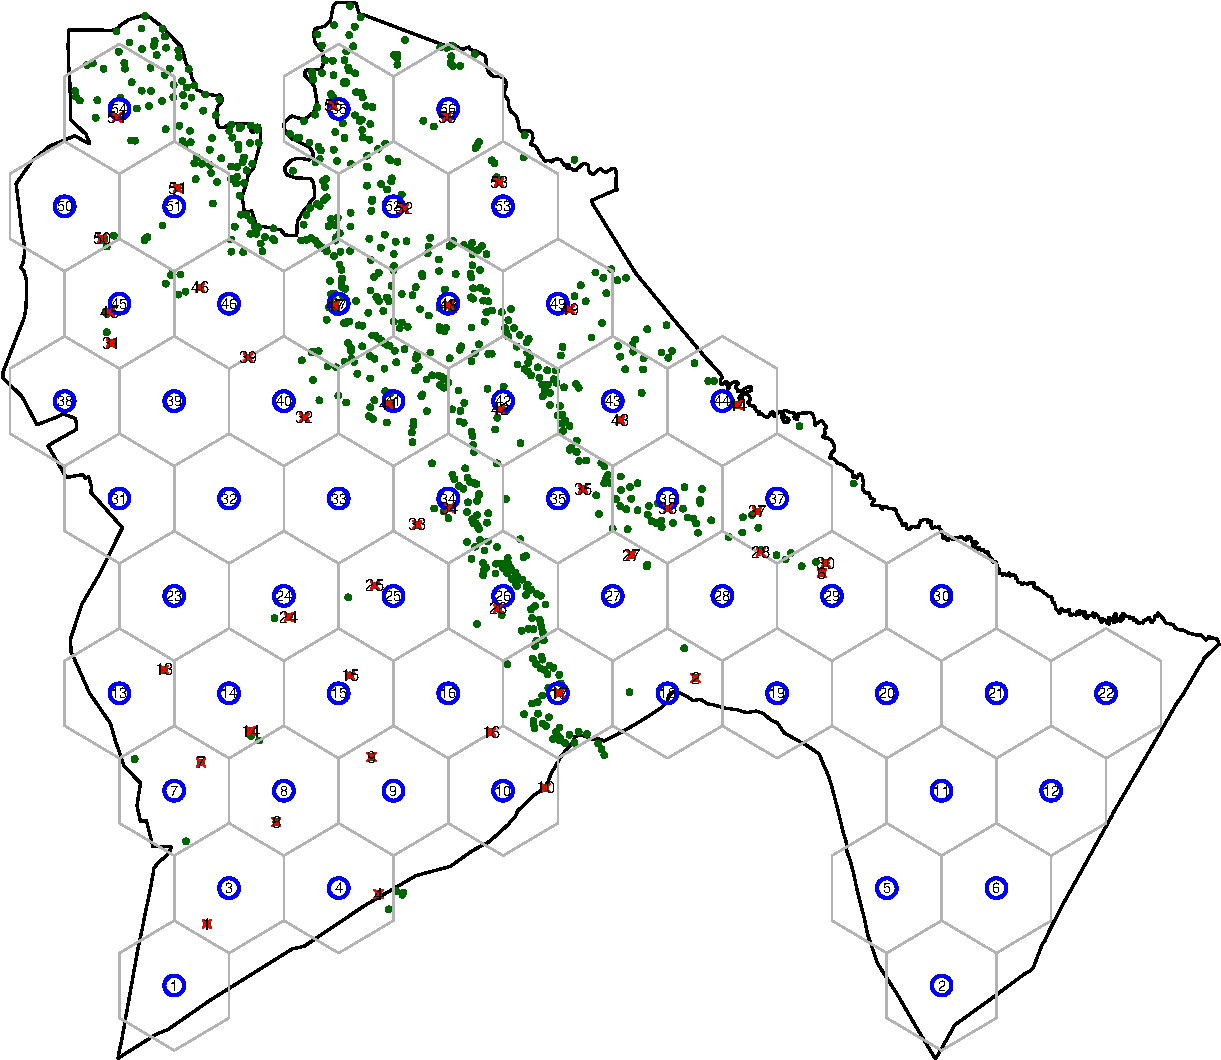
\includegraphics{notesS3Mtri_files/figure-latex/unnamed-chunk-17-1} 

}

\caption{Sampling map of Sennar at d = 15 kms}\label{fig:unnamed-chunk-17}
\end{figure}

~

In the map above, there are hexagons with more than one selected village
with one of them not ``local'' to the sampling point it is associated
with.

We might want to consider applying a more local search for the nearest
village. We can potentially do this by limiting the search for the
nearest village to within the hexagon of the sampling point. This will
be a minor edit of the nearest point algorithms that we currently have.


\end{document}
